\documentclass{article}
\usepackage[utf8]{inputenc}
\usepackage{url}
\usepackage{amsmath, amsthm, amssymb, amsfonts}
\usepackage{amssymb}
\usepackage{tikz,rubikcube,rubikrotation,rubikpatterns}
\usepackage{color}
\usepackage{floatrow}
\usepackage{listings}
\usepackage{apacite}
\lstset{ %
language=C++,                % choose the language of the code
basicstyle=\footnotesize,       % the size of the fonts that are used for the code
numbers=left,                   % where to put the line-numbers
numberstyle=\footnotesize,      % the size of the fonts that are used for the line-numbers
stepnumber=1,                   % the step between two line-numbers. If it is 1 each line will be numbered
numbersep=5pt,                  % how far the line-numbers are from the code
backgroundcolor=\color{white},  % choose the background color. You must add \usepackage{color}
showspaces=false,               % show spaces adding particular underscores
showstringspaces=false,         % underline spaces within strings
showtabs=false,                 % show tabs within strings adding particular underscores
frame=single,           % adds a frame around the code
tabsize=2,          % sets default tabsize to 2 spaces
captionpos=b,           % sets the caption-position to bottom
breaklines=true,        % sets automatic line breaking
breakatwhitespace=false,    % sets if automatic breaks should only happen at whitespace
escapeinside={\%*}{*)}          % if you want to add a comment within your code
}

\usepackage{caption}
\captionsetup[figure]{labelformat=empty}% redefines the caption setup of the figures environment in the beamer class.
\markright{\textsc{rubikcube} package; \hspace{2cm}file = main.tex}
%% increase textwidth to make room 
\addtolength{\oddsidemargin}{-1.5cm}
\addtolength{\textwidth}{3cm}
%% brace and bracket 
\newcommand{\Rubikbracket}[1]{$\left(\mbox{#1}\right)$}
\newcommand{\Rubikbrace}[1]{$\left\{\mbox{#1}\right\}$}
\author{ep15193}
\title{Rubiks Cube Project}\vspace{-50pt}
\date{October 2017}

\usepackage{physics}
\usepackage{mathtools}
\DeclarePairedDelimiter{\opair}{\langle}{\rangle}
\newtheorem{theorem}{Theorem}[section]
\newtheorem{lemma}[section]{Lemma}

\begin{document}
\maketitle


\medskip
The cube is made up out of 27 small cubes , referred to as cubies. These include the 8 corner cubies , 12 edge cubies and the 6 center ones with one non-visible 'cube' in the middle.
\vspace{-20pt}
\begin{figure}[h]
\floatbox[{\capbeside\thisfloatsetup{capbesideposition={right},capbesidewidth=4cm}}]{figure}{\caption{\textbf{Left (L), Up (U) and Right Moves (R)}}\label{cubemoves1}}
{
	\hspace{-10cm}
	\begin{tikzpicture}
	  \hspace{1cm}
      \RubikFaceUp   {}{W}{W} {}{W}{W} {}{W}{W}%
      \RubikFaceFront{}{O}{O} {}{O}{O} {}{O}{O}%
      \RubikFaceRight{G}{G}{G} {G}{G}{G} {G}{G}{G}%
      \ShowCube{2cm}{0.5}{\DrawRubikCubeRU}
      \RubikFaceUp   {}{}{} {}{}{} {}{}{}%
      \RubikFaceFront{}{}{} {O}{O}{O} {O}{O}{O}%
      \RubikFaceRight{}{}{} {G}{G}{G} {G}{G}{G}%
      \hspace{1cm}
      \ShowCube{2cm}{0.5}{\DrawRubikCubeRU}
      \RubikFaceUp   {W}{W}{} {W}{W}{} {W}{W}{}%
      \RubikFaceFront{O}{O}{} {O}{O}{} {O}{O}{}%
      \RubikFaceRight{}{}{} {}{}{} {}{}{}%
      \hspace{1cm}
      \ShowCube{2cm}{0.5}{\DrawRubikCubeRU}
     \end{tikzpicture}
}
\end{figure}
\begin{figure}[h]
\floatbox[{\capbeside\thisfloatsetup{capbesideposition={left},capbesidewidth=4cm}}]{figure}{\caption{\textbf{Face (F) , Back (B) and Down (D) Moves}}\label{cubemoves2}}
{
     \begin{tikzpicture}
     \hspace{-2cm}
      \RubikFaceUp   {W}{W}{W} {W}{W}{W} {}{}{}%
      \RubikFaceFront{}{}{} {}{}{} {}{}{}%
      \RubikFaceRight{}{G}{G} {}{G}{G} {}{G}{G}%
      \ShowCube{2cm}{0.5}{\DrawRubikCubeRU}
      \RubikFaceUp   {}{}{} {W}{W}{W} {W}{W}{W}%
      \RubikFaceFront{O}{O}{O} {O}{O}{O} {O}{O}{O}%
      \RubikFaceRight{G}{G}{} {G}{G}{} {G}{G}{}%
      \hspace{1cm}
      \ShowCube{2cm}{0.5}{\DrawRubikCubeRU}
      \RubikFaceUp   {W}{W}{W} {W}{W}{W} {W}{W}{W}%
      \RubikFaceFront{O}{O}{O} {O}{O}{O} {}{}{}%
      \RubikFaceRight{G}{G}{G} {G}{G}{G} {}{}{}%
      \hspace{1cm}
      \ShowCube{2cm}{0.5}{\DrawRubikCubeRU}
      \end{tikzpicture}
}
\end{figure}
\vspace{20pt}
\newline Above shows the 6 basic moves of the cube, to which the black cubies are transformed by rotating the specific face 90 degrees clockwise.  When applying one of these moves it is necessary to reference how to describe the change of the cubie. Fixing the cubies in the start configuration allows to reference cubicles ..............$\&\&\&\&\&\&\&\&\&$

 
\subsection*{Notes}	
Homomorphism to identity - we know there is one because there is a solved configuration.\newline

By FHT we know $G_{corner}/Z_{3} <= S_{8}$ the kernel is a normal subgroup of a group homomorphism , which is G corner.\newline

Can check individual moves correspond to 0 mod 3 , check symmetric groups on moves e.g. LR

RLUDFB

\subsection*{Introduction}

\paragraph*{}
\subsubsection*{History on the cube}
\cite{History}
The cube was first created by a Hungarian Professor named Erno Rubik. The original version is one which mimics the cube seen today including the coloured stickers. To him it wasn't meant to be a hobby or game like element, instead it was created to aid him in explaining three dimensional geometry. Although being the creator ,he found as he mixed up the cube and the stickers became jumbled he was unable to solve it.
\textit{It was a code I myself had invented!” he wrote. “Yet I could not read it.”}
Thus creating the phenomenon seen today, with a staggering 400 million sold and  1 in 7 people believed to have played with the cube. After this amount of time the cube has still not fallen out of popularity.With 'SpeedCube' competitions still rife the world record has been broken once more in 2017 amounting to 4.69 seconds to solve the 3 by 3 cube by Patrick Ponce (USA).\cite{Record}

Singmasters \cite{Magic}%
notation states that there are 6 basic moves of the rubiks cube (RLUFDB) which will be referenced throughout this project.
\subsubsection*{Possible and non possible moves}

The cube has 8 corner cubies have 3 faces while the 12 edge cubies have 2 faces leaving the 6 center cubies with a singular face. When applying one of these basic moves to the cube it's impossible for these center cubies to stray from the cubicle in which they live in.
So applying probability to the scenario , should allow to calculate the total number of configurations.
There is a choice of 8! positions for the corner cubies , and as there's 3 faces there are $3^8$ possible orientations. Similarly with the 12 edge cubies , combining these results give a total of $2^{12} * 3^8 * 8! * 12!$ $\approx 519$ quintillion configurations.
However what isn't known yet is which of these are actually possible from a set of permutations from the starting configuration.

\subsubsection*{Goal of the project}

This gives us motivation to see which of these configurations are not valid, why they're not valid......$\&\&\&\&\&\&\&\&\&$

\paragraph*{}


\subsection*{Important Theorems and Lemmas}

\paragraph*{}
\subsubsection*{Groups, Subgroups}

\subsubsection*{Group}
 
A group G is defined as a set with a binary operation $*$ such that , $* : G \ \ *\ \ G \rightarrow G$.
Which follows these properties.
\begin{itemize}
	\item It's closed under the operation $*$,  $\forall f, g \in G , f*g\ is\ also\ in \ G$
    \item The operation is associative so $for\ any\ f, g\ and\  h\ in\  G\ ,\  f*(g*h) = (f*g)*h$
    \item For every element in the group there exists an inverse, so for an element $ f\ \in\ G\ \exists\ g\ \in\ G\ such\ that\ f*g=e=g*f$
    \item The group contains an identity element $\epsilon \ such\ that\ for\ any\ f \in G\ f*\epsilon=\epsilon=\epsilon *f$
\end{itemize}

A homomorphism is a function $\phi $ from two groups G and H,  such that $\phi$ preserves the group operation 
\begin{equation}
	\phi(a*b)= \phi(a) * \phi(b)
\end{equation}

\subsubsection*{Example}
Group of multiplication $\in \ \mathbb{Z}$.
\newline The group definition is very useful when understanding following theorems and lemmas about the cube and can be applied directly below.

The group of the Rubiks Cube $(G,*)$ can be represented by the cube permutations, composed of the 6 basic moves of the cube listed previously.  This group will be a subset of size to the total configurations calculated in the Introduction as here the group actions (which can create a configuration) will be defined explicitly.

\textcolor{red}{EXPAND PROOF ,M be a set of moves 
\begin{itemize}
\item G is closed under *, 
\item e is the empty move , do nothing
\item if there is a move M then inverse is just reversing what you did
\item Associativity is more complex proof $\&\&\&\&\&\&\&$
\end{itemize}}


\subsubsection*{Normal Subgroup}
A subgroup H of G is normal if $ gH=Hg\ , \forall \ g \in \ G$ this is denoted as $H\trianglelefteq G$ and $H\triangleleft G$ if $G \neq H$

\subsubsection*{Automorphisms}
This is just any isomorphism which is a mapping from one object to itself. The set of all of these automorphisms in an object form the automorphism group.

\subsubsection*{Semi- Direct Product}
Given group G , subgroup H , normal subgroup $N \triangleleft G$ and that the following hold ,
\begin{itemize}
\item G is the product of subgroups G = NH where $N \cap H = {e}$ 
\item For every $g \in G \ , \exists unique \ h \in H and \ n \in N\ ,\ such that g=nh$
\item $\exists \ a \ homomorphism \ G \rightarrow H$ that is the identity on H whose kernel* is N.

\textit{*the kernel of a homomorphism is just the elements which map to the identity}
\end{itemize}

\subsubsection*{Wreath Products}

The Wreath products of two groups G and H below:.
\begin{itemize}
	\item $G^{H}$ is the set of all functions defined on H with values in G, where $G^{H}$ is an automorphism 
    \item Let X be a finite set , where $G^{X}$ is acted upon by H (this is just functions taking non identity values on a finite set of points X = $\{x_{1},x_{2},.. x_{p}\}$. So is trivially smaller than the set of all functions.
\end{itemize}
\begin{equation}
	G^{X} \wr  H = G^{X} \triangleleft H
\end{equation}
is then the wreath product of G and H. So is just the semi direct product of p copies of G by H.\cite{Wreath}

\paragraph*{}
\newpage
\subsubsection*{Alternating and Symmetric Groups}
Let X be a set and let S(X) be the symmetric group on X; the elements of S(X)
are the permutations of X (i.e. bijections $X\rightarrow X$) and the group operation is
composition of maps.
In contrast an Alternating group A(X) only contains the permutations to which are just even cycles, as opposed to the symmetric group above containing even and odd cycles.  For notation purposes these two groups will be defined as $A_{n} $and $S_{n}$. 


%Trivially the alternating group $A_{n}$ is contained in the kernel of the map , as it's the even cycles to which are the elements all are mapped to 0. (The kernel just gives the elements mapped to zero by the function).

A useful map to consider is an operation called a group homomorphism between two groups defined by the following properties:
%CITE GROUP THEORY NOTES

\begin{align*}
\phi : G\rightarrow H\ is\ a&\ homomorphism\ if: \\
& The\ map\ is\ a\ well-defined\ mapping \\
&\phi\ (ab)\ =\ \phi\ (a)\ *\ \phi\ (b)\ \forall\ a,b\ \in\ G\\
&im(\phi) = \{\phi(a) | a \in G\}\\
&ker(\phi)= \{a\in G |\phi(a) = e'\}
\end{align*}
In our case we can define a function as below which will map the elements of $S_{n}$ to either 1 or -1 in the cases outlined in the definition below.
\begin{equation}
\phi : S_{n} \rightarrow \{-1,1\} \qquad
  \phi(x)=\begin{cases}
    1, & \text{if x is an even number of transpositions}.\\
    -1, & \text{if x is an odd number of transpositions}.
  \end{cases}
\end{equation}
When x $\in \phi(x)$ equals 1, it means it can be expressed as an even number of transpositions. Transpositions are defined as the 2 cycle permutations, but to show the well-defined property of this map  we need to first show all permutations in $S_{n}$ can be written as a product of transpositions.%INSERTPROOF%% 
This can be shown by the following inductive argument.The base case for $S_{2}$ is trivial. Suppose any permutation of n takes less than n transpositions. Consider a permutation w of length n+1 (transpositions). Using the base case we can perform one transposition to swap the $n+1^{st}$ element in the correct place. Thus by the inductive hypothesis we have less than n transpositions for the remaining n elements , making the total less than n+1 transpositions. 
Now this is known the map can be shown to be a homomorphism by the following.

\begin{proof}
\item Our map can easily be verified to satisfy the conditions above. It is well defined , it can be expressed as some product of transpositions by the proof above.
\item Take two elements $\sigma , \tau \in S_{n}$. The goal is to show $S_{\tau\sigma} = S_{\tau}*S{\sigma}$
\item Either of these can be written like so $\sigma = \alpha_{1} ... \alpha_{a}$ ,$\tau = \beta_{1} ... \beta_{b}$, with some integers a and b factorisations of $\alpha$ and $\beta$ as a product of transpositions. 
\item $\sigma\tau = \alpha_{1} ... \alpha_{a}\beta_{1} ... \beta_{b}$ now expresses $\sigma\tau$ as a product of a+b transpositions. 
\item $\phi(\sigma\tau)\ =\ (-1)^{a+b}\ =\ (-1)^{a}(-1)^{b}\ =\ \phi(\sigma)\phi(\tau)$
\item thus conditions of homomorphisms are satisfied.
\end{proof}
As the map is known to be a homomorphism the kernel $ker(\phi)$ is of the form $\{a \in g|\phi(a) =e'\}$ where e' is the identity element of the set {-1,1}. For this case as the identity of this set cannot be 0 as a norm for groups such as $(\mathbb{Z},+)$,$(\mathbb{N},+)$ as the 0 element does not exist thus shall be defined at the elements of even cycles (odd transpositions). So we have $A_{n}\subset ker(\phi)$ but also it is the entire kernel itself so $A_{n} = ker(\phi)$ , if it wasn't then for some $S_{n} \notin A_{n} \in ker(\phi)$. However this cannot be the case as only even cycles are mapped to -1 , and any even cycles in $S_{n}$ are in $A_{n}$ by definition.
Taking into consideration the Group Homomorphism Theorem, or alternatively the First Isomorphism Theorem  
\begin{theorem}[Group Homomorphism Theorem]
\label{eq:5}
$G/ker(\phi)\ \cong\ im(\phi)$
\end{theorem}
Showing that the group G / by the kernel is isomorphic to the image of the group. Being isomorphic means there exists a homomorphism between the two groups which is also injective (one to one).
Substituting the values above defined for the kernel and the image of the group , it can be concluded that,  
\begin{equation}
S_{n}/A_{n} \cong \mathbb{Z}_{2}
\end{equation}
The cyclic group $\mathbb{Z}_{2}$ is placed at the end as it is equivalent to the set of $\{1,-1\}$ with just two elements, x and the identity (as x is the 1 and the identity has already been defined to be -1).
\paragraph{} From the Group Homomorphism Theorem there is now a new collection called a quotient group , but to understand what a quotient group is to groups one must first consider the left and right cosets formed by each corresponding group.	
With G a group and H a subgroup of G the left and right cosets are as follows:
\begin{itemize}
\item gH = $\{gh\ |\ h \in H\}$ is the left coset 
\item Hg = $\{hg\ |\ h \in H\}$ is the right coset 
\end{itemize}
The subgroup H is just the smallest group contained in G which generates all the elements of H. Taking H = $\{R\}$ (the right turn) as an example, H is now the subgroup of $\mathcal{G}_{RC}$ generated by all right turns as shown. 
\vspace{-20pt}
\begin{figure}[hbt]
\centering%
\hspace{-12cm}
\begin{tikzpicture}
  \RubikCubeSolved%
  \ShowCube{2cm}{\DrawRubikCubeRU}
    \hspace{.7cm}
    \quad\Rubik{R}%
    \hspace{.7cm}
  \RubikRotation{R}
  \ShowCube{2cm}{\DrawRubikCubeRU}
  	\hspace{.7cm}
    \quad\Rubik{R}%
    \hspace{.7cm}
   \RubikRotation{R}
   \ShowCube{2cm}{\DrawRubikCubeRU}
   	\hspace{.7cm}
    \quad\Rubik{R}%
    \hspace{.7cm}
   \RubikRotation{R}
   \ShowCube{2cm}{\DrawRubikCubeRU}  
\end{tikzpicture}%
\end{figure}
\vspace{20pt}
This is one instance of a right coset purely by definition on the original group $\mathcal{G}_{RC}$. It is such that whatever the size of the subgroup H it is identical to size of the coset. This is by construction as there is one element in the coset for each element in the subgroup.
It can also be said that any two coset from a subgroup H constructing from the group G, must be either distinct or the same. So any subgroup must have disjoint cosets , making them unique in definition. This can be shown by a simple proof by contradiction:
\begin{proof}
\item Suppose there were two right cosets Hx and Hy which share elements.
\item $h_{1}x$ = $h_{2}y$ for some $h_{1},h_{2} \in H$
\item taking inverses x = $h_{1}^{-1}h_{2}y$ , $h_{3} = h_{1}^{-1}h_{2}$
\item thus x = $h_{3}y$ and hx = $hh_{3}y$
\item so every element of Hx can be written as one of Hy
\item so every element of Hx is in Hy, thus Hx= Hy
\end{proof} These such right cosets will partition the rubiks cube group into equal sized disjoint sets. As the kernel of $\mathcal{G}_{RC}$ is a group itself, the number of distinct cosets is the size of the quotient $|G|/|ker(\phi)$. This is by Lagrange's Theorem.
\begin{theorem}[Lagrange's Theorem]
\label{Lagrange}
For H a subgroup of a group G , the size of H must be a divisor of the size of G.
So $x|H| = |G|$ for some $x\geq1$
\end{theorem}So now there is the quotient group $S_{n}/A_{n}$ is isomorphic to $\mathbb{Z}_{2}$ and of order dividing the rubiks cube group $\mathcal{G}_{RC}$ by Lagrange, now whats left is to show is that the map $\phi : S_{n}/A_{n} \rightarrow \{1,-1\}$ preserves an homomorphism as above. As the alternating group has been defined as the kernel above , the group operation (multiplication) will hold in a similar way to the $\phi : S_{n} \rightarrow \{1,-1\}$ map. There are 4 possible occurrences of multiplication in this map defined below.
\begin{align}
x\ is\ even,\ y\ is\ even\qquad	\phi(xy) = \phi(x)\phi(y) = 1*1 &= 1\\
x\ is\ even,\ y\ is\ odd\ \qquad	\phi(xy) = \phi(x)\phi(y) = 1*(-1) &= -1\\
x\ is\ odd,\ y\ is\ even\qquad	\phi(xy) = \phi(x)\phi(y) = (-1)*1 &= -1\\
x\ is\ odd\ ,y\ is\ odd \ \qquad	\phi(xy) = \phi(x)\phi(y) = (-1)*(-1*) &= 1
\end{align}
Note: By x is even , y is odd , it means for x to be defined as even number of transpositions , y to be odd number of transpositions.So homomorphic property of multiplication holds, thus map must be homomorphic.


%group $S_{n}/A_{n}$ is isomorphic to the set containing 0 and 1. As a further argument this set containing 0 and 1 is identical to saying the cyclic group $Z_{2}$, which contains either 0 (the identity), or 1.Group operation is defined similarly , and $({0,1}, +(mod2)) = Z_{2}$ , as two evens cycles still give an even \textcolor{red}{PROP A3 LATEST LINK PROVE}(e.g. 2=0mod2, 2+2=0mod2 ..) as well as any two odd cycles (1+1=2=0mod2) , which mean by group definition both will result to 0 in  the map defined, and 0 (identity) using modulus in $Z_{2}$.Note: this still complies with the definition that the kernel is just the alternating groups as any one even cycle can be written as the product of transpositions of two odd cycles.

While presently this may not seem that important this conclusion will be paramount in defining the analysis of the cube. This will be referenced later on in the project after valid configurations have been defined.
Now this theory can be related to the example of the 3 by 3 cube. Consider the move $DR^{-1}$ on the start configuration of the cube.\textcolor{red}{USE VIDEO EXPLANATION}


\vspace{-20pt}
\begin{figure}[hbt]
\begin{minipage}{3cm}%
\centering%
\begin{tikzpicture}[scale=0.5]
    \hspace{1cm}
  \RubikCubeSolved%
  \ShowCube{2cm}{0.5}{\DrawRubikCubeRU}
    \hspace{1cm}
    \quad\Rubik{D}%
    \hspace{1cm}
  \RubikRotation{D}
  \ShowCube{2cm}{0.5}{\DrawRubikCubeRU}
  	\hspace{1cm}
    \quad\Rubik{R}%
    \hspace{1cm}
   \RubikRotation{R}
   \ShowCube{2cm}{0.5}{\DrawRubikCubeRU}
\end{tikzpicture}%
\end{minipage}%
\end{figure}
\vspace{20pt}
Only considering the corner cubies for now, labeling them appropriately will allow for the moves to be expressed as a combination of disjoint cycles. The group considered when making these permutations is the group of all corner cubies $Z_{3}^{8}$. The labeling of the cube is as such \textcolor{red}{***INSERT LABELLING***}


\begin{figure}[h]
\centering
\begin{minipage}{3cm}%
\begin{tikzpicture}[scale=0.5]
  \RubikCubeSolved%
  \ShowCube{2cm}{0.5}{\DrawRubikCubeRU}
\end{tikzpicture}%
\end{minipage}%
\end{figure}




\newpage
\begin{equation}
D(\theta)= (1)(2)(3)(4)(5\ 6\ 7\ 8) \ \ \ \ \ \ \ R^{-1}(\theta)= (1\ 7\ 8\ 4)(2)(3)(5)(6)
\end{equation}

Are the cycles of the Down and Right inverse moves respectively which can be combined to obtain. 
\begin{equation}
DR^{-1}(\theta) = (1\ 8\ 4)(5\ 6\ 7)
\end{equation}

Now there is a cycle which alternates the position of the 6 cubies listed above. However this doesn't really achieve anything when looking to solve the cube, as far as the user is concerned this is just any random move $M \in G$. Aiming for a set of moves which oriented 2 cubies for instance would be far more useful in proving properties of the corner cubies and it's corresponding group $Z_{3}^{8}$. Taking the inverse of the move above, $D^{-1}R$, one obtains a similar disjoint cycle set of , 
\begin{equation}
D^{-1}R(\theta) = (1\ 7)(5\ 8)
\end{equation}


These cycles are in fact isomorphic , which there is a combination which actually achieves the aim. Through inspection applying the moves together the combination is as follows

\begin{equation}
(DR^{-1}D^{-1}R)^{2}  U^{-1}  (DR^{-1}D^{-1}R)^{4} U
\end{equation}
\vspace{-20pt}
\begin{figure}[h]
\centering
\begin{minipage}{3cm}%
\begin{tikzpicture}[scale=0.5]
  \RubikCubeSolved%
   \hspace{-1.2cm}
  \ShowCube{2cm}{0.5}{\DrawRubikCubeRU}
  \RubikRotation{D}\RubikRotation{Rp}\RubikRotation{Dp}\RubikRotation{R}
  \RubikRotation{D}\RubikRotation{Rp}\RubikRotation{Dp}\RubikRotation{R}
  \RubikRotation{Up}
  \RubikRotation{D}\RubikRotation{Rp}\RubikRotation{Dp}\RubikRotation{R}
  \RubikRotation{D}\RubikRotation{Rp}\RubikRotation{Dp}\RubikRotation{R}
  \RubikRotation{D}\RubikRotation{Rp}\RubikRotation{Dp}\RubikRotation{R}
  \RubikRotation{D}\RubikRotation{Rp}\RubikRotation{Dp}\RubikRotation{R}
  \RubikRotation{U}
  \hspace{1cm}
  \ShowCube{2cm}{0.5}{\DrawRubikCubeRU}

\end{tikzpicture}%
\end{minipage}%
\end{figure}
\vspace{20pt}


But this inspection doesn't seem very trivial and leaves the question why is this move above like so. For this explanation it's useful to turn to commutators from Group Theory. 
\begin{equation}
The\ commutator\ of\ two\ elements\ ,\ g\ and\ h\, of\ a\ group\ G\ ,\ is\ the\ \ element\ :\ ghg^{-1}h^{-1}
\end{equation}

For the cube this can be translated by setting g,h to be a specific set of moves. So really what's done above is to find the commutator which orients the two corner cubies by using the definition of a commutator. Where instead of considering disjoint cycles , defining g and h like so

\begin{equation}
	g = R^{-1}DRD^{-1}R^{-1}DR\ \ \ \ \ \ 
    h = U^{-1}
\end{equation}
and applying the commutator algorithm $(ghg^{-1}h^{-1})$ gives the set of moves to orient two corner cubies again. The importance of these commutators is high as it allows the user to gain intuition into actually solving the cube rather than just following a set algorithm. This also becomes particularly useful when the cube is a few moves off the start configuration and say the user needs to permute two corner cubies, now with the knowledge of the correct group commutator this can be achieved.



\subsection*{Context on Cube}
\subsubsection*{Generating and Minimally generating subgroups}


\subsubsection*{Generators}
Let G be a group , a subset $S\subseteq G$ is a generating set of G if $G =\langle S\rangle $. In other words every element of G can be written as a finite product (under group operation)  of elements of S. These elements are called generators of G.Taking the group G to be composed of the 6 basic moves  $G= \{{F,L,R,U,D,B}\}$, such that  any cube permutation can be made, allows  a comparison to be made of what a generator means to this specific example.  For example taking $S=\{R\}$ gives the subgroup which obtains all possible cube permutations obtained by rotating the right face $\{R,R^2,R^3,R^4\}$. As the order of a group is defined as either the least $n \in \mathbb{N}$ such that $g^n = \epsilon$ (where g is a member of the group),  or alternatively the size of the subgroup it generates, the order for S will be 4. Note it stops at $R^4$ as the group is cyclic* , so $R^5= R$.*by cyclic it just means to say that there exists an element which creates a generating set.\newline In group theory many groups share the property of being Abelian, which means for a group G if $\forall x,y\ \in\ G\ ,\ x*y=y*x$. One example could be $(\mathbb{Z},+)$ the group of the integers on addition, for any integer x,y this will hold (3+4 = 4+3) as the integers are commutative and associative in definition.
However applying this to the rubiks cube group this will not hold , showing us the order in which the moves are applied does in fact matter. This is shown by a simple case of the move M = $\{L,R2,D\}$ below

\vspace{-30pt}
\begin{figure}[h]
\centering
\begin{minipage}{3cm}%
\begin{tikzpicture}[scale=0.5]
  \RubikCubeSolved%
   \hspace{-1.2cm}
  \RubikRotation{L}\RubikRotation{R2}\RubikRotation{D}
  \ShowCube{2cm}{0.5}{\DrawRubikCubeRU}
  \RubikCubeSolved%
  \RubikRotation{R2}\RubikRotation{D}\RubikRotation{L}
  \hspace{1cm}
  \ShowCube{2cm}{0.5}{\DrawRubikCubeRU}
\end{tikzpicture}%
\end{minipage}%
\end{figure}
\vspace{20pt}
Where , from the starting configuration, the left hand cube has been applied the sequence ${L,R2,D}$ and the right hand cube ${R2,D,L}$. Visually one can see the are obviously not equal , thus breaking the condition of what it means to be abelian.This is because these moves share common cubies, a move consisting of opposite faces alone such as R,L would hold commutativity (RL=LR) however for the whole cube this can't be said. So clearly some elements of the group commute while others do not.\newline The set of elements to which the generators are made from is defined as the generating set. These generators are a useful way for defining groups , however for large groups such as the rubiks cube it can become difficult to gain information due to the sheer enormity of possible generators. When talking about these commuting element is often useful to mention orbits and their stabilisers. 

Given the definition of an orbit from Group Theory ,
\begin{equation}
\begin{aligned}
if\ G\ acts\ on\ a\ set\ A\ ,\ then\ the\ orbit\ of\ a \in A\ (under\ this\ action)\ is\ the\ set\ \{\ a*g\ :\ g \in G\} \\
The\ stabiliser\ of\ an\ orbit\ is\ \{g\in G | g*x = x\}\ the\ set\ of\ all\ elements\ that\ fix\ x
\end{aligned}
\end{equation}

From the definition the orbit is just the subset of A which can be moved by any move from G, with A being the total number of configurations of the cube. As said above the center cubies always stay in the 6 center positions hence will always be in the same orbit. This applies to the corner and edge cubies as well (relative to corner and edge positions). 
From properties of an orbit , it must be either disjoint or the same (this can be shown from a single contrapositive argument). So one could consider 3 separate orbits within the Cube where,

\begin{equation}
A = A_{x}\cup A_{e}\cup A_{c}\cup A_{e}
\end{equation} 
$A_{x}$ are the center pieces, $A_{e}$ edge pieces and $A_{c}$ the corner pieces. We know any of these respective cubies will stay under their respective positions from a move G, but what isn't so is trivial is when considering the whole set of the cubies. Moreover prove how any group action from the Rubiks Group $\mathcal{G}_{R}$ preserves any resulting configuration will be in the same orbit.\cite{Harvard} 
An example of when the wouldn't apply is any illegal configuration of the cube (e.g. from pulling pieces out, switching stickers etc.) ,defining the difference into what is and isn't a valid configuration is key in proving the statement about same orbits above. This will be referenced later in the paper.
Orbits aswell as describing how points, or in the case described, cubies move can also be used to compute stabilisers. These can be the subgroups of elements which fix one or more points, which can be very useful in solving the cube in a step by step solution.\cite{PermGroups}

Suppose there was an algorithm which took a given scrambled state to the starting configuration. Where in this algorithm one piece has been permuted correctly, call it $G_{1}$, where the rest of the cube remains to be solved. These subsequent permutations will aim to put their respective pieces in the correct place (and orientation) without disturbing the previous permutation.   

This algorithm is called a stabiliser chain where the first permutation fixing the first piece of the cube , $G_{1}$ shall be defined as the stabiliser of the chain.  $G > G1 > G2 > .... > Gn = I$, where I is the identity (starting configuration).Each of these $G_{i}'s$ should contain a set of moves which solves the i'th piece, therefore one of the move sequences for that $G_{i}$ will be in $G_{i+1}$, a permuation in $G_{i}$ will always lie in $G_{i+1}$. In other terms with a list  of a move $a_{i1},a_{i2},a_{i3}, ...$ every $b \in G_{i} \in a_{ik}G_{i+1}$ for some k. So $G_{i}$ is made up entirely of the set of all cosets $a_{i1}G_{i+1}, a_{i2}G_{i+1}, a_{i3}G_{i+1}, ... $ for every k. There now exists a way to find the generators for $G_{i+1}$ a specific sequence solving the i+1'th piece, that given the generators of $G_{i}$ and the list of move sequences $a_{ik}$ (or coset representatives), the new stabiliser chain can be built.\cite{Schreier}

The rubiks cube group $\mathbb{G}_{RC}$ if to be implemented by a computer using each individual configuration , which is $(8!*3^8*12!*2^12/3*2*2) \approx 4.3*10^{19}$, becomes computationally inefficient to try and store each sequence for each configuration.The aim of implementing this algorithm however is to identify the groups composition structure by using subgroups to factorise the problem down, to solve the cube from a given state. The algorithm in question the Schreier Sims Algorithm, is given motivation from the Schreier Lemma on subgroups.

\begin{lemma}[Schreier Lemma on Subgroups]
Let G be a group with a set of generators S. Let H be a subgroup of G, and let A be the set of coset representatives of H $\in$ G. For any g $\in$ G, let g denote the element of A that represents the coset gH.\newline Then H is generated from the set $\{(sa)^{-1} (sa) | a \in R, s \in S \}$. 
\end{lemma}

\begin{proof}
Take any $h\in H (\in G)$ , h = $s_{1}s_{2}...s_{k}$ for some sequence of generators $s_{i} \in S$.
\[Let\ \ \ t_{i} = s_{i+1}...s_{k}\ \ \ be\ the\ coset\ representative\ for\ the\ s\ sequence\] , this is such that $t_{0}$ = $s_{1}...s_{k}$ = h and $t_{k}$ defines the identity $t_{k} = e$.
Rewriting h with new set of coset representatives t gives h = $(t_{0}^{-1} s_{1} t_{1}) ...(t_{k-1}^{-1} s_{k} t_{k})$.
We also find that $(s_{i} t_{i})H = s_{i}(t_{i} H) = s_{i} ( s_{i+1}..s_{k} H) = (s_{i}s_{i+1}..s_{k})H = t_{i-1} H so s_{i} t_{i} = t_{i-1}.$
Rewriting h with this new condition gives h = $((s_{1} t_{1})^{-1} s_{1} t_{1})((s_{2} t_{2})^{-1} s_{2} t_{2}) ...((s_{k} t_{k})^{-1} s_{k} t_{k})$.
By definition t is the set of coset representatives, giving each i interval a factor of $s_{i}^{-1}s_{i}$. Any element $h \in H$ is a product of these factors , thus the set $\{(sa)^{-1} (sa) | a \in R, s \in S \}$ will generate H.\\
\end{proof}
The method to factorise into smaller subgroups uses a combination of Lagranges Theorem with the Orbit Stabiliser Theorem, 
\begin{theorem}[Orbit Stabiliser Theorem]
.\\
$|G|= |Gx|*|G_{x}|$\\
applying Lagrange\\
$|Gx|=|G/G_{x})|=|G:G_{x}|$
\end{theorem}
which simply states the size of the orbit of the group can be retrieved from the size of the group partitioned by its stabilisers. Any subgroup chain can also be completed in $log_{2}|G|$ as the stabiliser is a subgroup for the rubiks cube group (G $G>G_{x})$ meaning $[G:G_{x}]\geq 2$, so $|G|\geq2|V|$ and $|G|\geq 2^{k}.$
\cite{OrbStab}. So reducing the problem logarithmically can cause a major difference to understanding an algorithm to solve the cube in a certain state in the orbit, however the reduction is not that significant as $[G:G_{x}]$ still remains very large. In fact for each predecessing $G_{i}$ the number of generators grows exponentially, $G_{1}$ = 6*24, $G_{2}$=6*24*22 ... For an efficient solver you would need to extract which of these generators are useful to the solving problem as a large number of these are not. The algorithm has been adapted to improve on these flaws , which along with other solvers shall be mentioned later.
%Incremental Schreier-Sims algorithm.



%INSERT SOMETHING MAYBE ABOUT 2X2 CUBES ON THE REFERENCE


\pagebreak
\subsubsection*{Possible and Non Possible Configurations}


We have the orientations of a corner cubie defined as $Z_3$.
This is because each of corner cubie has 3 coloured faces which can be oriented differently. 
This makes the set of 8 corner cubies the product of all these different permutations.\[\mathcal{Z}_{3}^8 = \prod_{i=1}^{8}\mathcal{Z}_{3}\]
To think about the different orientations of a cubie the idea is to fix a 'starting orientation' .We know there must exist a homomorphism which takes the cubies to the correct orientation , as there exists a set of moves leading any valid configuration to the start configuration (solved). Thus using the group $Z_{3}^{8}$ , generators of such group would be basis elements,  so fixing 7 cubies  give us the homomorphism below: 

\begin{align}
	\delta : G \Rightarrow G && \delta\mathcal({Z}_{3}^{7}) = \epsilon
\end{align}

Also when considering the subgroups of $G_{RC}$ it's necessary to define another subgroup along with the orientations of the cubies, this being $S_{8}$ the permutation group of 8 elements (the 8 corner cubies). This can be defined like such , as taking any corner cubie on the cube it has 3 faces as described above which can all be alternated between each other. This being equivalent to a 3-cyclic group , denoted $C_{3}$. Which leads again to a product of 8 groups \[\mathcal{C}_{3}^8 = \prod_{i=1}^{8}\mathcal{C}_{3}\], where $C_{3}^{8}$ is denoted as $S_{8}$.These 2 definitons above analogously follow a similar argument when considering the 12 edge cubies along the cube $Z^{12}_{2}$.
\paragraph*{}
Going back to orbits and considering the difference between correct configurations , we can start by giving notation on what defines a valid configuration.At any configuration all corner cubies , as well as edge cubies, should be on orientation number corresponding to that of their group. That is,
\begin{align*}
e.g. x_1&=0, x_2=2 ...,x_8=1\\
y_1&=1, y_2=1 ... , y_12=0
\end{align*}
One must also define a sign variable which states what the move has done to change where the arrangement of the corner cubies or that of the edge cubies. 
Define $\tau (\in S_{8})$ as the sign of the corner cubies and $\delta (\in  S_{12})$ as the sign of the edge cubies. This sign is 1 if there is an even number of transpositions, which are 2 cycle permutations, and -1 if there is an odd number. 
\begin{equation}
  \tau(x)=\begin{cases}
    1, & \text{if x contains an even number of transpositions}.\\
    -1, & \text{if x contains an odd number of transpositions}.
  \end{cases}
\end{equation}
\textcolor{red}{DEFINE K CYCLE PERM}

Ignoring the center cubies as they always stay in the same position relative , a configuration is defined as \textbf{$(\tau,\delta, x, y)$ }.
For example an invalid configuration would be that below:

\newcommand{\invalidseq}{[invalidseq],F2,F2}%
\newcommand{\invalidseqarrow}{$\quad\overrightarrow{\strut\textsc{invalidseq}}\quad$}

\begin{figure}
\centering
  \RubikCubeSolved%
  \ShowCube{2cm}{0.5}{\DrawRubikCubeRU}\invalidseqarrow
  \RubikRotation{\invalidseq}
  \RubikFaceUp   {W}{W}{W} {W}{W}{W} {W}{W}{G}%
  \RubikFaceFront{O}{O}{W} {O}{O}{O} {O}{O}{O}%
  \RubikFaceRight{O}{G}{G} {G}{G}{G} {G}{G}{G}%
  \ShowCube{2cm}{0.5}{\DrawRubikCubeRU}
\end{figure}
\vspace{20pt}
This is because there exists no set of moves to obtain the configuration shown on the right. The change of orientation of one singular cubie (from the start configuration) can only be achieved by breaking the cube ,so is invalid. Given our definitions of a configuration and the labelling previous \textcolor{red}{REFERENCE LABEL ABOVE} this can be shown mathematically. 

%To show this apply the following:

To see if one configuration can be found from another is identical to saying $(\tau^{'} ,\delta^{'} , x^{'} , y^{'} )$ = $(\tau,\delta, x, y)$ * M e.g. applying a move M gives the different configuration. Using knowledge of orbits, define it to be the set of all possible configurations from the Rubiks Cube group G. It's known whenever a move M applied to a possible configuration is also valid then one can conclude any other valid configuration can be found from a move M. As this trivially holds for any one of the basic moves $M= \{{F,L,R,U,D,B}\}$ one can conclude using basic inductive principles, that for any intermediate set of moves this will still hold as the configuration will still be in the orbit. Giving reason to saying any valid configuration of the cube can be solves with a specific set of moves. However to prove one of the fundamental theorems on the cube we still need to look at the corresponding signs of two correct configurations, hence we define the two following maps. 


\begin{equation}
\phi_{corner}: G \rightarrow S_{8}\quad \quad 
\delta_{corner}: G \rightarrow S_{12}
\end{equation}
This map all elements of the group to the subgroup $S_{8}$ (Symmetric group of the corner cubies). This map is a homomorphism as it is trivially well defined, and preserves the group operation of a move e.g. $\phi (L*L) = \phi (L) * \phi(L)$. With this homomorphism the above objective , $(\tau,\delta, x, y) \longrightarrow (\tau^{'},\delta^{'}, x^{'}, y^{'})$ from $\tau^{'} = \tau\phi_{corner}(M) $ , and similarly with edge pieces $\delta^{'} = \delta\phi_{edge}(M) $ works as from the following proof:\newline We know that the homomorphism is surjective, otherwise there would exist possibles moves in $M= \{{F,L,R,U,D,B}\}$ taking corner cubies out of subset of corner cubie positions (contradicting our definition of the orbit of the cube group). This trivially cannot happen , a cubie with 3 faces cannot live in an edge cubie consisting of 2 faces, meaning any application of $\phi_{corner}: G \rightarrow S_{8}$ will result in one of the 8 corner cubies. In having a surjective homomorphism , the Group Homomorphism Theorem can be applied once again \eqref{eq:5} by inspection the kernel of this group is empty thus the image is equivalently $S_{8}$. Any $\tau$ $\in S_{8}$ of this new image subgroup (S8) can be described as an element which moves the corner cubies from their start positions to the new positions. From the way $\tau$ is defined it shall be either 1 or -1, using the homomorphic properties of $S_{8}$ must contain an inverse element (for every element in the group), meaning applying one of the basic moves M we can get cubie A to its original position from its new position. One of these basic moves, moves 4 corner cubies , making the permutation a 4 cycle thus being an odd number of transpositions $\tau^{'}$ = -1 and thus doing $(\tau^{'} ,\delta^{'} , x^{'} , y^{'} )$ = $(\tau,\delta, x, y)$ * M means $\tau^{'} = \tau\phi_{corner}(M)$. So if $\tau^{'} \neq \tau$ e.g. $\tau = 1$ applying M means $\tau$ will now alter from an even to an odd number of transpositions thus $\tau$ = 1 * -1 and sgn($\tau^{'}$) = sgn($\tau$).\newline There is an analogous argument with the edge cubies for $\delta^{'} = \delta\phi_{edge}(M) $. Combining the analogous argument and the fact that any basic move M moves 4 corner and 4 edge cubies the following can be concluded:
\begin{proof}
\begin{align*}
sgn(\tau^{'}) sgn(\delta^{'}) &= sgn(\tau)sgn(\delta) \\ 
		&= sgn(\tau)sgn(\phi_{corner}(M))sgn(\delta)sgn(\phi_{edge}(M))&&\text{Using homomorphisms above}  \\
        &= sgn(\tau)(-1)sgn(\delta)(-1) &&\text{Both 4 cycles}  \\
        &=  sgn(\tau)sgn(\delta)  &&\qedhere
\end{align*}
\end{proof}
Furthermore as the start configuration is defined as (1,1,0,0) by looking at the definition of the sgns thus any other valid configuration is also in the start configuration as shown above giving that $sgn(\tau) = sgn(\delta)$. 
This fact is fundamental in cube theory, but a full definition of what makes a correct configuration is not fully complete. For this conservation of parity between edge and corner cubies must be verified. This touches on the point made earlier in the section discussing that each cubie , edge or corner, must be associated with a number to describe the orientation of the cubie in that specific cubicle, otherwise mathematically speaking , it cannot be told if the cubes are facing in the right directions. These x and y values must obey the following rules: 

\begin{equation}
\Sigma x_{i} =0mod(3) \qquad \Sigma y_{i} =0mod(2) 
\end{equation}

From the labelling defined previously for $x_{1}$ to $x_{8}$ and $y_{1}$ to $y_{12}$ the basic move M will change these values on one configuration($(\tau^{'} ,\delta^{'} , x^{'} , y^{'} )$ = $(\tau,\delta, x, y)$ * M) in the table below\cite{chengroup}:

\begin{center}
    \begin{tabular}{ | l | p{12cm} |}
    \hline
    Move & x' and y' value \\ \hline
    D &  $x_1,x_2,x_3,x_4,x_8,x_5,x_6,x_7$ \\
& $y_1,y_2,y_3,y_4,y_5,y_6,y_7,y_8,y_{10},y_{11},y_{12},y_9$\\ \hline
    R &  $x_1,x_7 +1,x_2 +2,x_4,x_5,x_6,x_8 +2,x_3 +1$\\ & $y_1,y_7,y_3,y_4,y_5,y_2,y_{10},y_{8},y_{9},y_{6},y_{11},y_{12}$\\ \hline
    U &  $x_2,x_3,x_4,x_1,x_5,x_6,x_7,x_8$ \\ & $y_4,y_1,y_2,y_3,y_5,y_6,y_{7},y_{8},y_{9},y_{10},y_{11},y_{12}$\\ \hline
    L & $x_4 +2,x_2,x_3,x_5 + 1,x_6 +2,x_1 + 1,x_7,x_8$ \\
& $y_1,y_2,y_3,y_5,y_12,y_6,y_{7},y_{4},y_{9},y_{10},y_{11},y_{8}$\\ \hline
    F &  $x_6 +1,x_1 +2,x_3,x_4,x_5,x_7 +2,x_2 +1,x_8$\\
& $y_1,y_2,y_8 +1,y_4,y_5,y_6,y_{3}+1,y_{11}+1,y_{9},y_{10},y_{7}+1,y_{12}$\\ \hline
    B &  $x_1,x_2,x_8 +1,x_3 + 2,x_4 + 1,x_6,x_7,x_5 +2$ \\
&$y_6 +1,y_2,y_3,y_4,y_1 +1,y_9 +1,y_{7},y_{8},y_{5}+1,y_{10},y_{11},y_{12}$\\ \hline
    \end{tabular}
\end{center}
The method in which the corresponding x's and y's have been added by a number between mod 2 or mod 3 is defined below. Assume the below cube consists of a valid configuration , where there exists a move sequence which rotates the top front face corner cubie in its cubicle only. 

\newcommand{\rotatecorner}{[rotatecorner],F2,F2}%
\newcommand{\rotatecornerarr}{$\quad\overrightarrow{\strut\textsc{rotate corner }}\quad$}
\begin{figure}[hbt]
\centering
  \RubikCubeSolved%
  \RubikFaceUp   {X}{X}{X} {X}{X}{X} {X}{X}{G}%
  \RubikFaceFront{X}{X}{W} {X}{X}{X} {X}{X}{X}%
  \RubikFaceRight{O}{X}{X} {X}{X}{X} {X}{X}{X}%
  \ShowCube{2cm}{0.5}{\DrawRubikCubeRU}\rotatecornerarr
  \RubikRotation{\rotatecorner}
  \RubikFaceUp   {X}{X}{X} {X}{X}{X} {X}{X}{W}%
  \RubikFaceFront{X}{X}{O} {X}{X}{X} {X}{X}{X}%
  \RubikFaceRight{G}{X}{X} {X}{X}{X} {X}{X}{X}%
  \ShowCube{2cm}{0.5}{\DrawRubikCubeRU}\rotatecornerarr
  \RubikFaceUp   {X}{X}{X} {X}{X}{X} {X}{X}{O}%
  \RubikFaceFront{X}{X}{G} {X}{X}{X} {X}{X}{X}%
  \RubikFaceRight{W}{X}{X} {X}{X}{X} {X}{X}{X}%
  \ShowCube{2cm}{0.5}{\DrawRubikCubeRU}
\end{figure}
\vspace{20pt}
Also assume the cubie fits in the cubicle correctly in the first cube , e.g. its in the correct position and orientation currently. Each time a move is applied and the cubie is rotated in a clockwise manner from it's correct orientation there will be an addition of 1 to preserve notational parity. For example let the cubie = $x_2$, when rotate corner sequence is applied the orange moves to the white facet clockwise 1 face, so the new $x_2^{'}$ becomes $x_2 + 1$. If the sequence was applied twice to go from the first to the third the new $x_2^{'}$ becomes $x_2 + 2$ as there are 2 clockwise movements. This is also similar for the edge pieces, but for only 2 changing faces there will only ever be a +1 or +0 (cycles back).
As an example the front face turn is shown below.


%INSERT DIAGRAM OF FRONT MOVE



\begin{figure}[hbt]
\centering
\RubikCubeSolvedWY
\RubikRotation{\sixspot}
\ShowCube{5cm}{0.5}{
	\DrawRubikCubeSF
	\node (x1) at (.5, 2.5)
		[black]{\small\textsf{x1}};
	\node (x2) at (2.5, 2.5)
		[black]{\small\textsf{x2}};
	\node (x6) at (.5, .5)
		[black]{\small\textsf{x6}};
	\node (x7) at (2.5, .5)
		[black]{\small\textsf{x7}};
}
\Rubik{F}%
\hspace{.5cm}
\ShowCube{5cm}{0.5}{
	\RubikRotation{F}\DrawRubikCubeSF
	\node (x6) at (.5, 2.5)
		[black]{\small\textsf{x6}};
	\node (x1) at (2.5, 2.5)
		[black]{\small\textsf{x1}};
	\node (x7) at (.5, .5)
		[black]{\small\textsf{x7}};
	\node (x2) at (2.5, .5)
		[black]{\small\textsf{x2}};
}
\caption{F move on solved cube}
\end{figure}

\paragraph*{}
\newpage
\subsection*{Possible Extension- CRAN cubing package}

For the section relating gods number and efficiency to actually solving the cube, it will be implementing the CRAN cubing package (seesource). From this it will
aid in the explanation about ways to solve the cube as well as showing how the mathematics behind the cube ties in with the programming.
After installing the CRAN package and using the R command to further access specific packages within CRAN , the cube functions can finally be accessed. The notation of defining the cube in terms of an array is as such:

\begin{figure}[h]
	\centering
	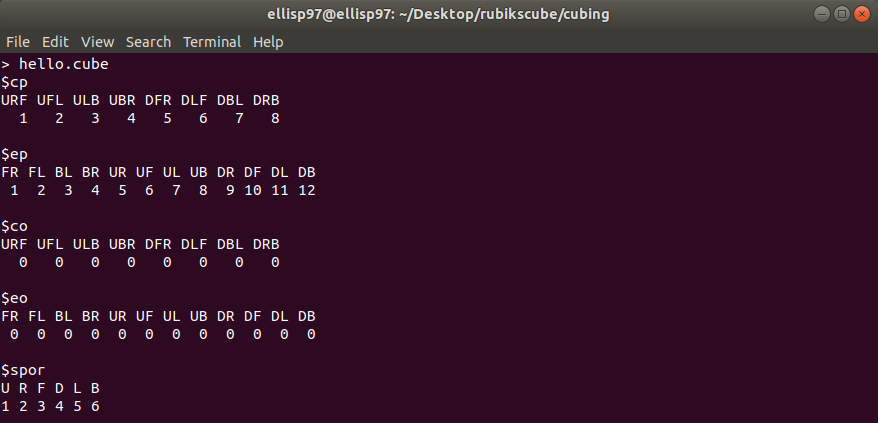
\includegraphics[scale=.75]{terminalcube.png}
\end{figure}
Entering the command hello.cube displays how the cube is stored with a similar notation to how it's labelled earlier in the project. Where \textbf{cp,ep,co,eo} stand for corner/edge permutation and orientation (where the cubicles live in the cubie).
\paragraph*{}
\textcolor{red}{INSERT SOME SORT OF CAMPRISON TO DO WITH LABELLING}
\paragraph*{}
Visual aid however is important as without this it becomes hard to see what's actually happening to the cube. This comes in 2d and 3d plots, with the commands plot(yourCube) and plot3d(yourCube) once defined(To enable the use of a 3D plot with RGL, start the RGL device in the R command).

\begin{figure}[h]
	\centering
	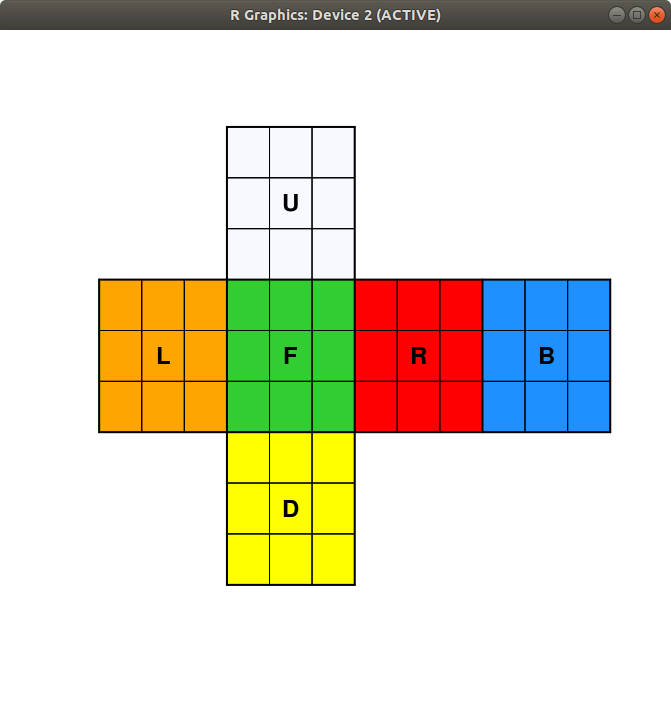
\includegraphics[scale=.4]{2dcube.png}
    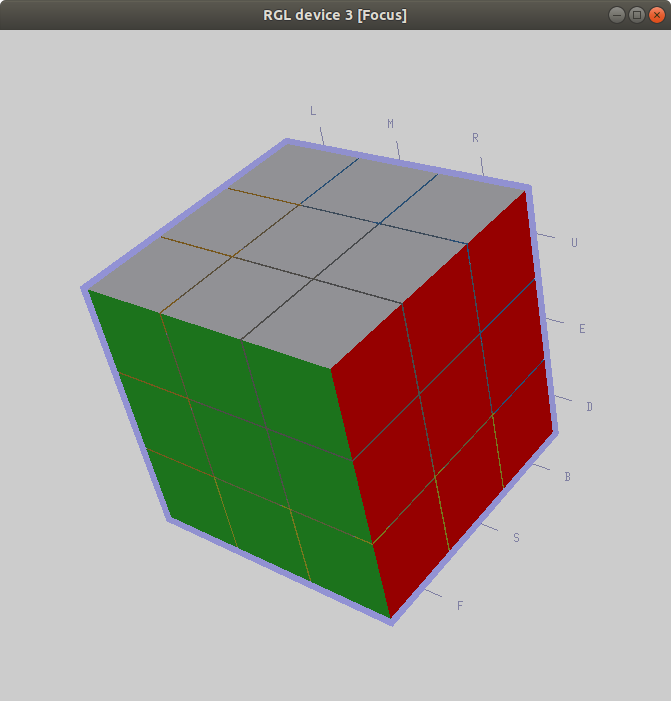
\includegraphics[scale=.4]{3dcube.png}
\end{figure}
\newpage
Using a construction like so allows the user to input any configuration of a cube into the system, whether it's valid or invalid (in terms of solvability defined previously) so long as it obeys methods of input e.g.

\begin{lstlisting}
>yourCube = cubieCube("UUUUUUUU RLLRRLLR BBFFFFBB DDDDDDDD LRRLLRRL FFBBBBFF")
>plot(yourCube, numbers = TRUE)
\end{lstlisting}
and then can plot in usual way (including numbers = TRUE displays the cubie positions on the cube like so).
\begin{figure}[h]
	\centering
	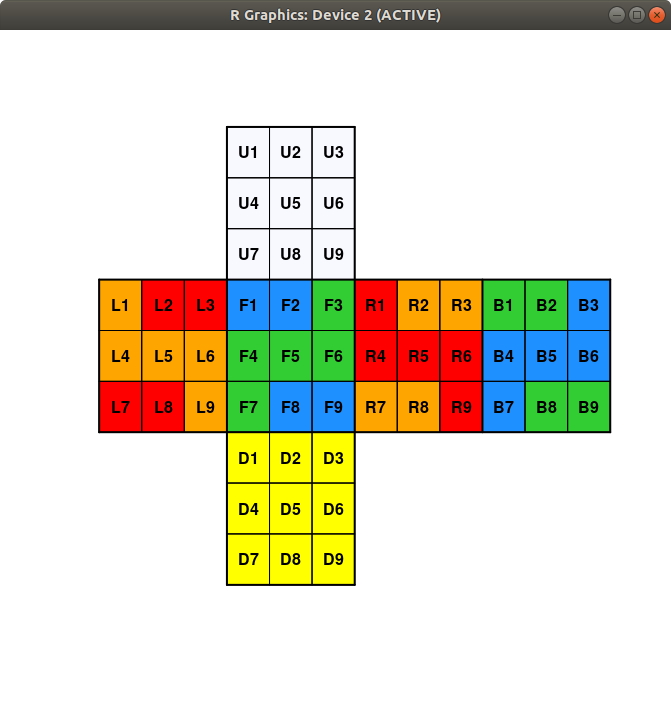
\includegraphics[scale=.45]{labelledcube.png}
\end{figure}
A function which is imperative for the input of these cubes is \textbf{is.solvable}. When on input of a cube previously defined will return a boolean value depending on whether the configuration entered is correct or not.
\paragraph*{}
\textcolor{red}{INSERT LINK ON AMOUNT OF FALSE CUBIES WITH TRUE CUBIES USING FUNC(sum(sapply(randCube(100, solvable = FALSE), is.solvable))) , USING COMBINATORIAL ARGUMENT}
\paragraph*{}
Furthermore when a cube which has an invalid configuration has been input, 
\begin{lstlisting}
>is.solvable(yourCube, split = TRUE)

  parity  co     eo
  TRUE   TRUE  FALSE
\end{lstlisting}
is solvable will tell you the condition of how yourCube fails to be solvable.
\paragraph*{}
\textcolor{red}{INSERT LINK TO HOW THIS RELATES TO MOD 3 STUFF}
\paragraph*{}
Using the following command a user can create their own move by separating the standard moves with spaces (or even separate lines). This has uses and can be used in conjunction with the is.solvable to see if a certain set of moves can take one configuration to the start configuration (solved).
\begin{lstlisting}
> yourCube <- getMovesCube(scan(what = character()))

1: D2 F2 U F2 D R2 D B L' B R U L R U L2 F L' U
20:
19 moves read

> mv <- scan(what = character())
1: D2 F2 U F2 D R2 D B L' B R U L R U L2 F L' U
20:
19 moves read

> result <- move(yourCube, mv)
> is.solved(result)

[1] TRUE
\end{lstlisting}
\paragraph*{}
\textcolor{red}{INSERT STUFF RELATING ON ANIMATION E.G. WR MOVE ANIMATE(ACUBE,MV)}
\paragraph*{}

A question must be asked on the efficiency of this 'solver', how it works and how fast it can be done. 
The solver used in the is.solvable function is called the \textit{Kociemba Solver}. This algorithm was created by Herbert Kociemba in 1992 which is an adapted version of the Thistlethwaite algorithm often referred to as the breakthrough for cube solvers \cite{Thistlethwaite}. So to understand how efficiency works between solvers this algorithm must be considered first.

\subsubsection*{Thistlethwaite's Algorithm}

The idea of this was to create a \textit{Divide and Conquer} style implementation, which essentially means to divide one big problem (solving the cube) into many different smaller subproblems. It uses the main concepts of group theory explained above, while utilising complex computer searches on very large lookup tables. 
The cube group $\mathcal{G}_{RC}$is split up into the following sequence of subgroups.  

\begin{equation}
  \mathcal{G}_{RC}=\begin{cases}
    G_{0} = \text{$\opair{L,R,F,B,U,D}$}.\\
    G_{1} = \text{$\opair{L,R,F,B,U^{2},D^{2}}$}.\\
    G_{2} = \text{$\opair{L,R,F^{2},B^{2},U^{2},D^{2}}$}.\\
    G_{3} = \text{$\opair{L^{2},R^{2},F^{2},B^{2},U^{2},D^{2}}$}.\\
    G_{4} = \text{1}.
  \end{cases}
\end{equation}

This technique allows the cube to be solved in a maximum of 52 moves. Using the smaller subgroups he restricts the possible space of moves which can be made, this works by moving down the chain of $G_{0}$ to $G_{4}$

\newpage

\bibliographystyle{apacite}
\bibliography{rc}

\end{document}

